\subsection{Automated SOS tests}
As indicated by the other team, the Automated SOS service is based on: a schedule job executed every 24 hours to send request regarding the usage of the ASOS service to the elderly people (over 60 years old). To avoid waiting so much time, we did a little modification on the source code of the project. One class called "src/data4help/src/main/java/avila/schiatti/virdi/Main.java" has to be modified:
\begin{itemize}
\item Substitute the code
\begin{verbatim}
	ASOSRequestScheduler.create()
\end{verbatim}
with
\begin{verbatim}
	ASOSRequestScheduler.create().setPeriod(10).setTimeUnit(TimeUnit.SECONDS)
\end{verbatim}
\item Add the import of the class TimeUnit on the top of the class
\begin{verbatim}
	 import java.util.concurrent.TimeUnit;
\end{verbatim}
\end{itemize}
After this modification, we still could not test the functionality of ASOS. Then after the other team fixed the bug, we tested it and we saw that the new user received a pending requests from Automated SOS. This test regarding UC13 has been done manually due to some unknown problem in JMeter (no new requests were found). 
\begin{itemize}
\item UC13 regards the creation of ASOS Request to elderly people
\end{itemize}

\begin{figure}[H]
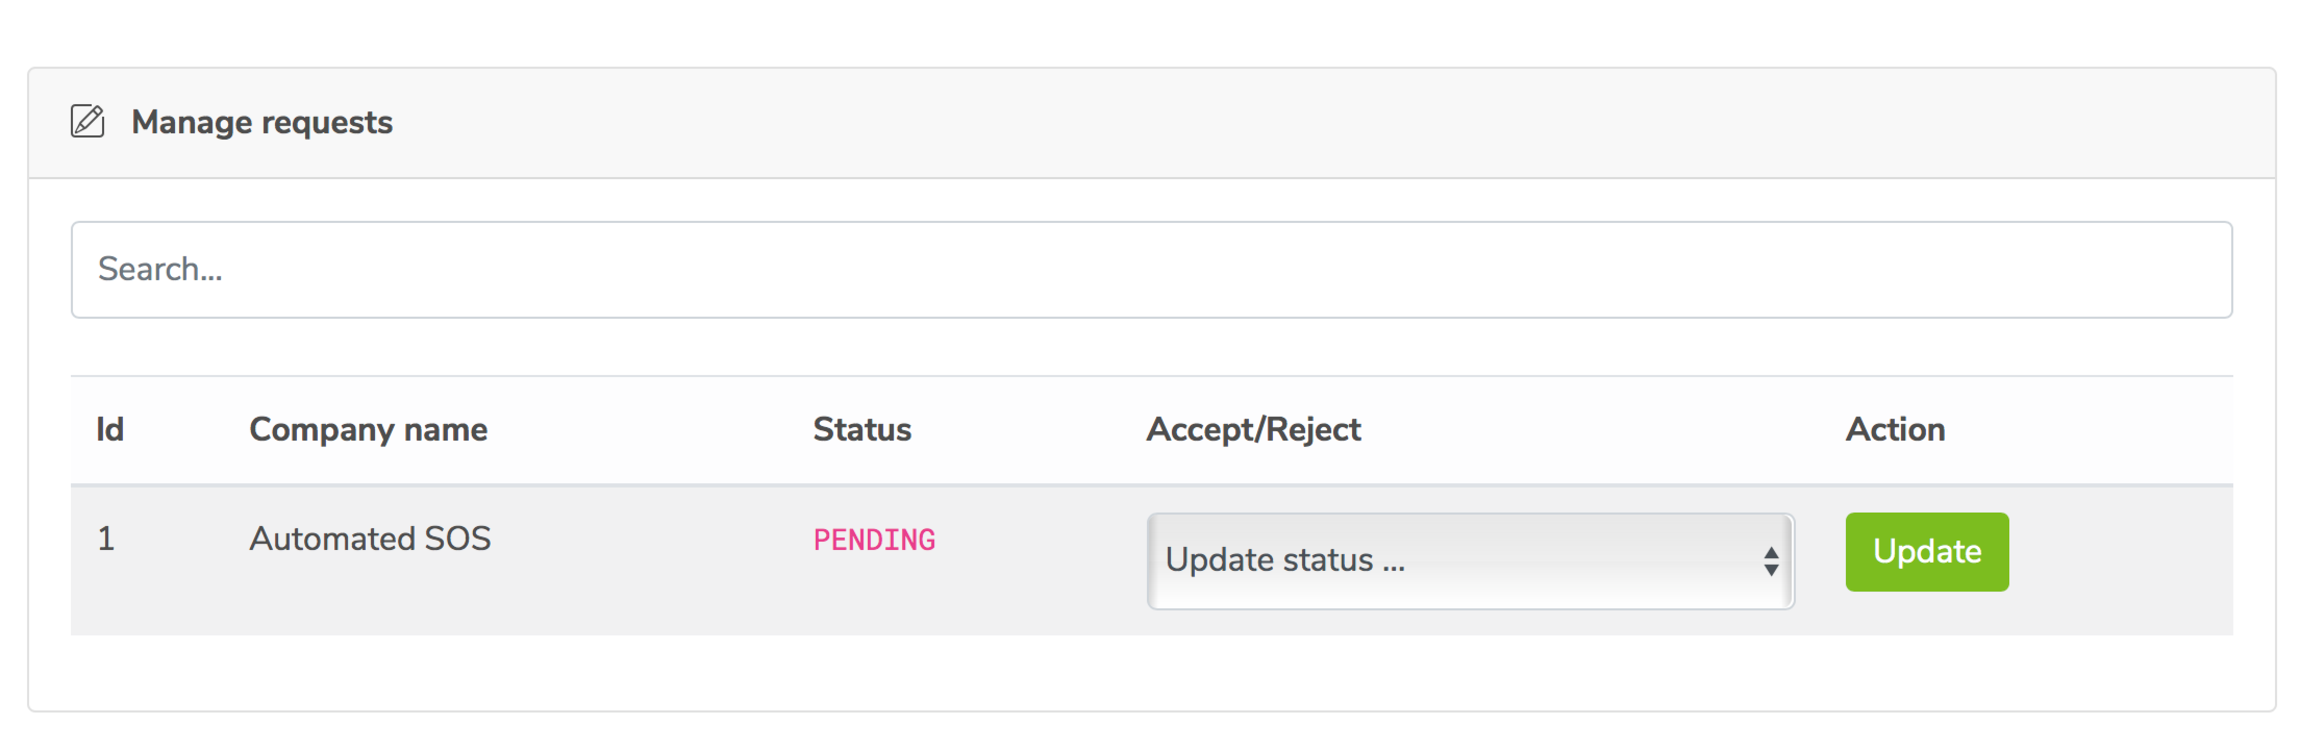
\includegraphics[width=\linewidth]{images/pendingASOS}
\caption{ UI Received ASOS requests }
\label{fig:asosrequest}
\end{figure}

The other UC14, UC15 and UC16, regarding receiving health data, sending health data and contacting emergency point, cannot be checked since the send of data cannot be done manually.
